\chapter{Ekologi Perilaku}\label{ch:b3:behavioural-ecology}

Seekor meerkat berdiri di atas gundukan rayap sementara anggota kelompoknya menggali
makanan, dan ketika seekor elang muncul ia menyalak lalu yang lain berlari ke
liangnya. Sang penjaga telah menghabiskan sejam tanpa makan lalu menjadikan
dirinya hewan yang paling mencolok di gurunnya. Mengapa? Seekor merak menyeret
sebuah ekor yang berongkos seperlima anggaran tenaganya lalu memperlambat pelariannya
dari harimau. Seekor lebah madu yang pulang dari sebuah ladang menari pada sebuah
sisir tegak, dan sudut tariannya terhadap tegaknya adalah sudut
makanannya terhadap mataharinya. Seekor gelatik besar yang memburu ulat di sepetak dedaunan
meninggalkannya selagi masih ada ulat yang dapat ditemukan. Tidak satu pun hewan
ini telah membaca bab ini, namun masing-masing berperilaku seolah-olah telah memecahkan sebuah
pengoptimalan, sebuah permainan, atau sebuah masalah dalam penghitungan kekerabatan. Ekologi
perilaku adalah kajian perilaku sebagai sehimpunan penyelesaian yang berevolusi:
untuk apa sebuah perilaku, menurut gen yang disebarkannya, dan berapa
ongkos serta manfaatnya agar seleksi alam menghasilkannya.
Perkakasnya adalah perkakas yang dipakai seorang ekonom --- pengoptimalan, \omterm{prop:b3:behavioural-ecology:hawk-dove}{teori
permainan}, penghitungan kekerabatan --- dan ujinya adalah lapangannya.

\section{Empat pertanyaan dan mesin naluri}

\begin{definition}[Pertanyaan Tinbergen]\label{def:b3:behavioural-ecology:tinbergen}
\index{empat pertanyaan Tinbergen}\index{pola tindakan tetap}%
\index{rangsang tanda}\index{pematrian}\index{masa kritis}
Tinbergen (1963) mengatakan sebuah keterangan lengkap tentang perilaku mana pun harus menjawab
empat pertanyaan: \emph{mekanisme}-nya (rangsang dan mesin saraf apa yang
menghasilkannya), \emph{perkembangan}-nya (bagaimana ia timbul pada individunya,
dari gen dan pengalamannya), \emph{fungsi}-nya (bagaimana ia menyumbang pada
ketahanan hidup dan perkembangbiakannya), serta \emph{sejarah evolusi}-nya (bagaimana ia
timbul dari perilaku leluhurnya). Para etolog yang merumuskannya telah
menegakkan kedua yang pertama. Banyak perilakunya berupa \emph{pola tindakan
tetap}: yakni urutan baku yang dilepaskan sebuah \emph{rangsang tanda} yang
sederhana lalu dijalankan sampai tuntas begitu dimulai --- seekor angsa abu-abu menggulirkan sebuah
telur yang tergeser kembali ke sarangnya dengan paruhnya, lalu merampungkan gerakannya
bahkan bila telurnya disingkirkan di tengah jalan; seekor anak camar herring mematuk sebuah bintik
merah pada benda berbentuk paruh mana pun, lalu mematuk lebih banyak pada sebuah tongkat bergaris merah
tiga daripada pada kepala seekor camar sungguhan; seekor ikan duri jantan menyerang apa pun yang
merah di bawahnya, termasuk sebuah van pos yang lewat yang dilihatnya lewat
jendelanya. Yang lain dipelajari di dalam sebuah jendela: \emph{pematrian}, yang dengannya
seekor anak angsa pada hari pertamanya mengikuti lalu sesudahnya memperlakukan sebagai induknya
apa pun yang bergerak --- seekor angsa, Lorenz, sebuah kotak kardus --- bersifat cepat,
tak terpulihkan, dan terbatas pada sebuah \emph{masa kritis}; pembelajaran nyanyian pada
burung, yakni contoh jilid Tahun~2, punya bentuk yang sama. Dikotomi
bawaan dan terpelajarnya keliru: sebuah perilaku punya sebuah acara genetik
yang menentukan apa yang harus dipelajari, kapan, dan dari siapa, dan
acaranyalah yang berevolusi.
\end{definition}

\begin{proof}[Bukti eksperimental]
Percobaan lapangan Tinbergen menetapkan caranya. Tawon penggali
(\emph{Philanthus}) pulang ke sebuah sarang yang tersembunyi di dalam pasir; ia memindahkan sebuah cincin
runjung pinus yang telah ditaruhnya di sekeliling satu pintunya sementara tawonnya pergi,
lalu tawonnya mencari pusat cincin yang tergeser itu --- ia telah mempelajari
tetenger tanahnya. Camar berkepala hitam menyingkirkan cangkang telur dari sarangnya sesudah
penetasannya; ia menata telur di samping cangkang bercat, cangkang alami, dan
benda lain, lalu mencacah mana yang diambil gagaknya: permukaan dalam
yang putih sebuah cangkang menarik pemangsa, dan penyingkiran yang tampak
seperti kerapian itu ternyata penyamaran. Percobaan anak camarnya mengukur sebuah
\omterm{def:b3:behavioural-ecology:tinbergen}{rangsang tanda} dengan menawarkan kepala kardus yang meragamkan satu ciri pada satu
waktu. Angsa Lorenz yang terpatri mengikutinya seumur hidup; bebek yang terpatri
pada hari pertamanya pada sebuah kotak yang bergerak sesudahnya tidak dapat dibuat
mengikuti seekor bebek.
\end{proof}

\begin{omfigure}
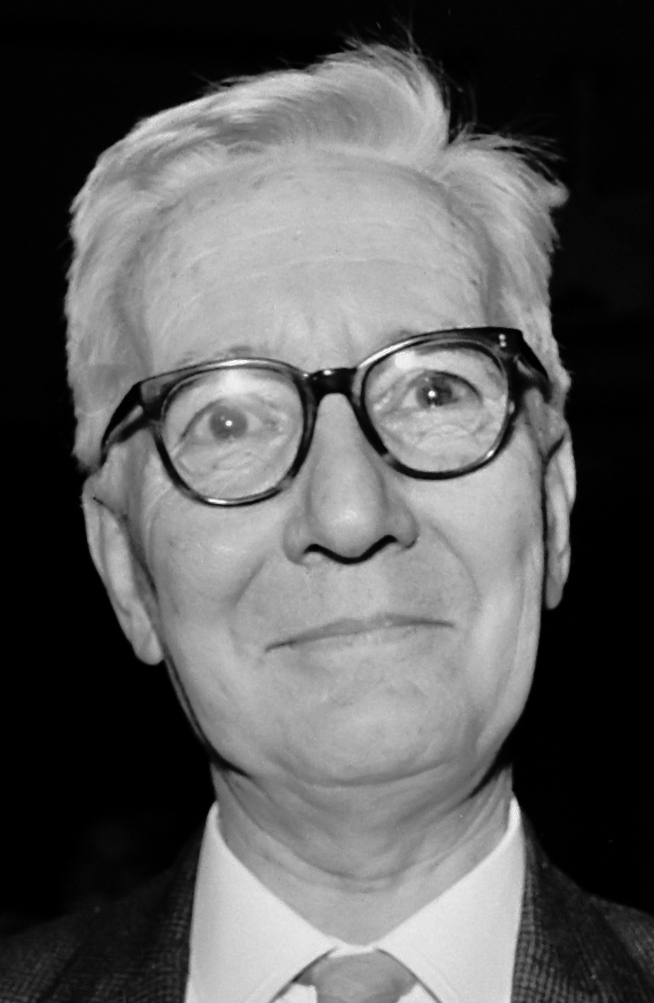
\includegraphics[width=0.36\linewidth]{images/book5/tinbergen.jpg}\hspace{0.04\linewidth}
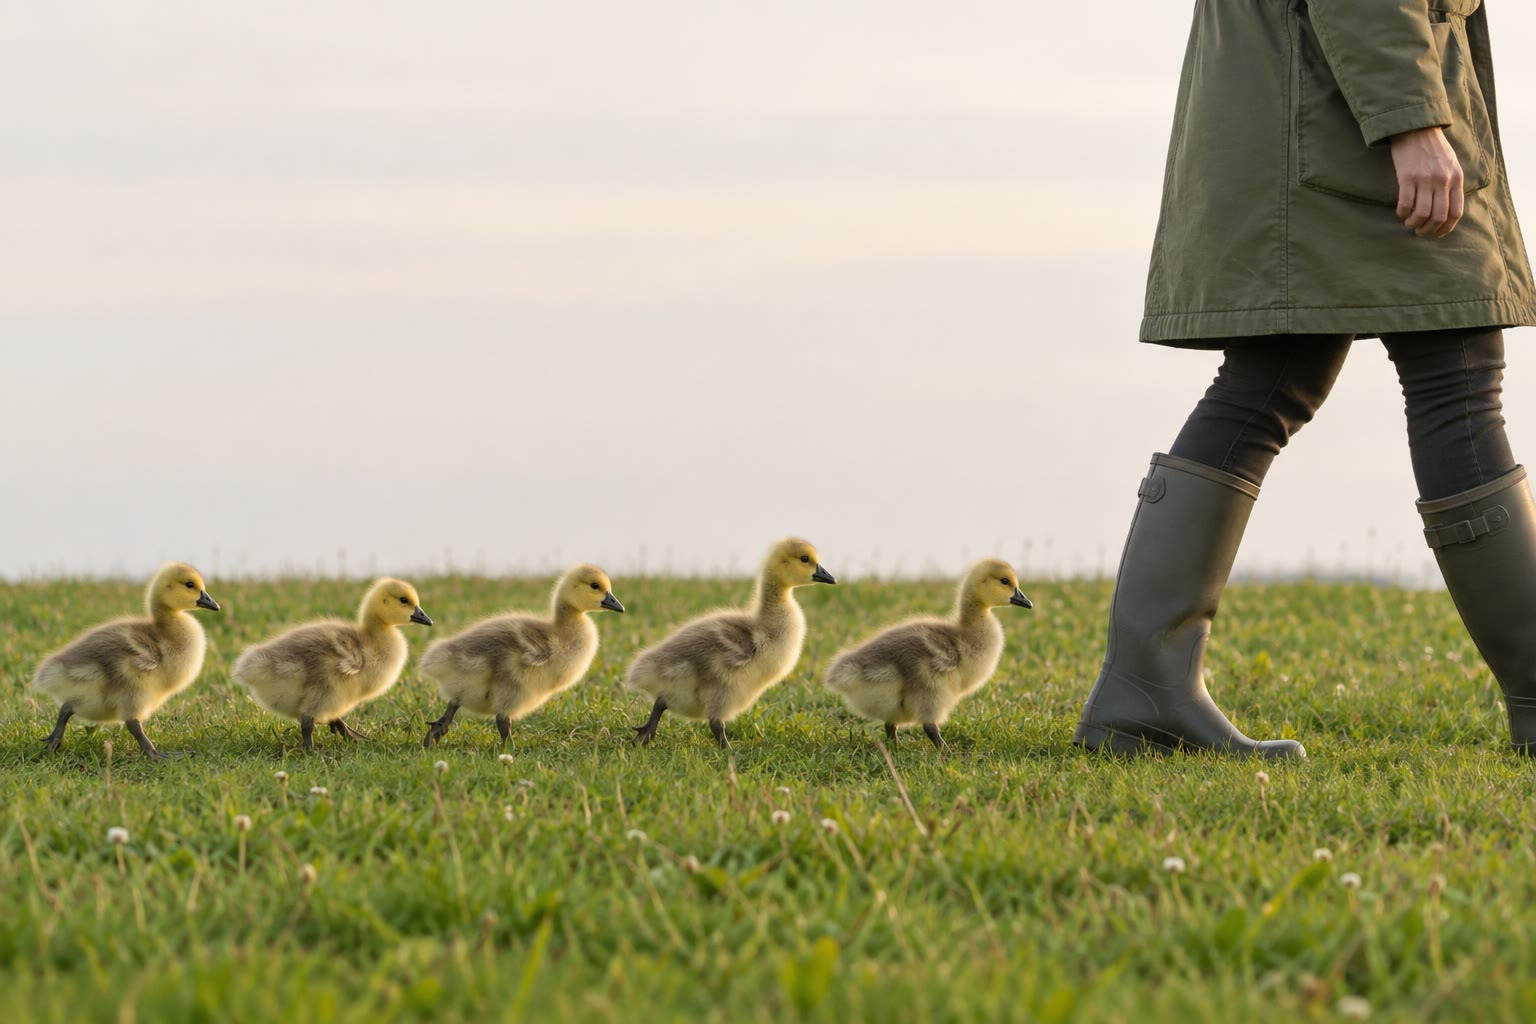
\includegraphics[width=0.52\linewidth]{images/book5/ai/b5-26-goose-imprinting.jpg}

{\small Kiri: Niko Tinbergen (1907--1988), yang membawa pertanyaan
perilaku ke lapangan lalu menjadikannya percobaan (foto
oleh Rob Mieremet, Anefo, 1973, CC0). Kanan: anak angsa yang mengikuti benda besar
pertama yang bergerak yang dilihatnya, sehari sesudah menetas, dan sesudah itu tidak pernah dibujuk
sebaliknya.}
\end{omfigure}

\section{Memutuskan: mencari makan yang optimal}

\begin{theorem}[Teorema nilai marginal]\label{thm:b3:behavioural-ecology:mvt}
\index{mencari makan yang optimal}\index{teorema nilai marginal}%
\index{waktu tinggal di petak}\index{mata uang}
Seekor pencari makan mengunjungi petak makanan yang terpisah oleh waktu perjalanan $\tau$. Di dalam sebuah
petak ia memperoleh tenaga $g(t)$ sesudah waktu $t$, dengan $g$ naik dan
cekung (petaknya terkuras). Bila ia meninggalkan tiap petaknya sesudah waktu $t$,
laju perolehan jangka panjangnya adalah $R(t) = g(t)/(\tau + t)$, dan waktu tinggal
$t^{*}$ yang memaksimumkannya memenuhi
\[
g'(t^{*}) = \frac{g(t^{*})}{\tau + t^{*}} = R(t^{*}) :
\]
tinggalkanlah sebuah petak ketika laju perolehan seketikanya di dalamnya telah turun ke
laju rata-rata di seluruh habitatnya, termasuk perjalanannya (Charnov,
1976). Akibatnya: makin lama waktu perjalanannya, makin lama tinggalnya
dan makin tuntas tiap petaknya terkuras; di dalam sebuah habitat yang lebih kaya
($R$ yang lebih tinggi) tiap petaknya ditinggalkan lebih cepat dan kurang terkuras; dan semua
petaknya ditinggalkan pada laju marginal yang sama apa pun mutunya, sehingga
sebuah petak yang miskin ditinggalkan nyaris seketika dan yang kaya hanya ketika ia
telah digarap turun ke rata-rata habitatnya. Bagi $g(t) = A(1 -
\mathrm{e}^{-t/T_{0}})$ syaratnya menjadi $(\tau + t^{*})/T_{0} =
\mathrm{e}^{t^{*}/T_{0}} - 1$, yang diselesaikan secara numeris: dengan $\tau = T_{0}$,
$t^{*} \approx 1.15\,T_{0}$; dengan $\tau = 4T_{0}$, $t^{*} \approx
2.0\,T_{0}$.
\end{theorem}
\begin{proof}
$R(t) = g(t)/(\tau + t)$; $R'(t) = [g'(t)(\tau + t) - g(t)]/(\tau +
t)^{2} = 0$ memberi $g'(t^{*}) = g(t^{*})/(\tau + t^{*})$. Secara geometris:
petakanlah $g$ terhadap $t$ dengan titik asalnya pada $-\tau$; $R(t)$ adalah kemiringan
garis dari $(-\tau, 0)$ ke $(t, g(t))$, yang maksimal tempat garis itu
menyinggung kurvanya --- dan itulah syaratnya. Sebuah $\tau$ yang lebih besar memindahkan
titik asalnya ke kiri dan titik singgungnya ke kanan; sebuah habitat yang lebih kaya mencuramkan
singgungnya lalu memindahkannya ke kiri. Bagi eksponensialnya, $g' = (A/T_{0})
\mathrm{e}^{-t/T_{0}}$ dan $g/(\tau + t) = A(1 - \mathrm{e}^{-t/T_{0}})/
(\tau + t)$; menyamakan lalu menata ulangnya memberi persamaan yang dinyatakan, dan
menyulihkan $t^{*} = 1.15T_{0}$ dengan $\tau = T_{0}$: kirinya $2.15$, kanannya
$\mathrm{e}^{1.15} - 1 = 2.16$.
\end{proof}

\begin{omfigure}
\begin{tikzpicture}
\begin{axis}[
  width=0.68\linewidth, height=5.8cm,
  axis x line=middle, axis y line=left,
  xmin=-4.5, xmax=5, ymin=0, ymax=1.15,
  xlabel={waktu (satuan $T_{0}$)}, ylabel={tenaga yang diperoleh di petaknya},
  xlabel style={font=\small, at={(axis description cs:0.95,0.0)}, anchor=north}, ylabel style={font=\small},
  tick label style={font=\small}, xtick={-4,-1,0,1.15,2}, xticklabels={$-4T_0$,$-T_0$,0,$1.15$,$2.0$}, ytick={0.5,1}, yticklabels={$0.5A$,$A$},
  clip=false,
]
\addplot[very thick, omDef, domain=0:5, samples=80] {1-exp(-x)};
\draw[thick, omThm] (axis cs:-1,0) -- (axis cs:1.55,1.13);
\draw[thick, omMeth!70!black] (axis cs:-4,0) -- (axis cs:3.5,1.081);
\fill[omThm] (axis cs:1.15,0.6834) circle (2pt); \fill[omMeth!70!black] (axis cs:2,0.8647) circle (2pt);
\draw[dashed, gray] (axis cs:1.15,0) -- (axis cs:1.15,0.6834); \draw[dashed, gray] (axis cs:2,0) -- (axis cs:2,0.8647);
\node[font=\scriptsize, omThm, anchor=north west, align=left] at (axis cs:-4.4,1.1) {perjalanan pendek, $\tau = T_{0}$:\\tinggalkan pada $t^{*} = 1.15\,T_{0}$,\\petaknya terkuras \qty{68}{\%}};
\node[font=\scriptsize, omMeth!70!black, anchor=north west, align=left] at (axis cs:2.4,0.62) {perjalanan panjang, $\tau = 4T_{0}$:\\tinggalkan pada $t^{*} = 2.0\,T_{0}$,\\terkuras \qty{86}{\%}};
\node[font=\scriptsize, omDef, anchor=north west] at (axis cs:3.0,0.86) {$g(t) = A(1 - \mathrm{e}^{-t/T_{0}})$};
\node[font=\scriptsize, gray, anchor=south] at (axis cs:-2.5,0.02) {perjalanan};
\end{axis}
\end{tikzpicture}

{\small \omterm{thm:b3:behavioural-ecology:mvt}{Teorema nilai marginal} yang digambar. Kurva perolehannya mendatar seiring
terkurasnya petaknya; garis dari awal perjalanannya ke sebuah titik pada
kurvanya berkemiringan sama dengan laju perolehan keseluruhannya; waktu terbaik untuk
pergi adalah tempat garis itu menyinggung. Sebuah perjalanan yang lebih panjang memindahkan titik asalnya
ke kiri dan titik singgungnya ke kanan.}
\end{omfigure}

\begin{proof}[Bukti eksperimental]
Cowie (1977) membiarkan gelatik besar memburu ulat tepung yang tersembunyi di dalam cangkir
berisi serbuk gergaji di dalam sebuah kandang burung, dengan waktu perjalanan antarcangkirnya diatur
lewat memasang tutup yang lebih lama atau lebih cepat dilepas; burungnya tinggal
lebih lama di tiap cangkirnya ketika perjalanannya lebih lambat, menjejaki ramalan teoremanya,
lalu melampauinya sedikit pada arah yang dijelaskan oleh memperhitungkan
ongkos tenaga perjalanannya. Burung jalak yang mengusung larva lalat
kepada anaknya (Kacelnik, 1984) mengambil muatan yang lebih besar dari pengumpan
yang ditaruh lebih jauh, sekali lagi sebagaimana dituntut penyelesaian pemaksimum laju bagi sebuah
kurva pemuatan. Tidak satu pun ujinya membuktikan bahwa burungnya menghitung
singgungan; keduanya menunjukkan bahwa seleksi telah menghasilkan kaidah praktis yang
hasilnya dekat ke optimumnya.
\end{proof}

\section{Perlawanan: teori permainan}

\begin{proposition}[Elang--Merpati dan siasat mantap secara evolusi]\label{prop:b3:behavioural-ecology:hawk-dove}
\index{teori permainan}\index{permainan Elang--Merpati}%
\index{siasat mantap secara evolusi}\index{seleksi bergantung-kekerapan}
Ketika perilaku terbaiknya bergantung pada apa yang dilakukan yang lain, tidak ada optimum,
hanya sebuah \emph{permainan}. Dua hewan memperebutkan sebuah sumber daya bernilai $V$; sebuah
\emph{Elang} bertarung sampai terluka (ongkos $C$) atau menang, sebuah \emph{Merpati}
memamerkan diri lalu mundur bila diserang. Rata-rata hasilnya adalah
\[
\begin{array}{c|cc}
 & \text{lawan Elang} & \text{lawan Merpati}\\ \hline
\text{Elang} & (V - C)/2 & V\\
\text{Merpati} & 0 & V/2
\end{array}
\]
Sebuah \emph{\omterm{prop:b3:behavioural-ecology:hawk-dove}{siasat mantap secara evolusi}} (Maynard Smith dan Price, 1973)
adalah siasat yang, begitu lazim, tidak dapat diserbu alternatif langka mana pun.
Bila $V > C$, Elang adalah SME-nya: bertarung berbalas bahkan melawan petarung. Bila $V
< C$, tidak ada siasat murni yang mantap --- sebuah populasi Merpati
diserbu Elang, yang memenangkan tiap perlawanannya, dan sebuah populasi Elang oleh
Merpati, yang menghindari lukanya --- dan SME-nya adalah memainkan Elang dengan
peluang
\[
p^{*} = \frac{V}{C},
\]
atau, secara setara, sebuah populasi yang pecahan itu berupa Elang. Pada
SME-nya kedua siasatnya sama baiknya, masing-masing rata-rata $V(1 -
V/C)/2$, yakni kurang daripada $V/2$ yang akan dibagi sebuah populasi Merpati:
perlawanannya merugikan semua orang, dan tidak ada yang dapat berbuat lebih baik sendirian. Seleksi
di sini bersifat \emph{bergantung-kekerapan}: kebugaran sebuah siasat turun ketika ia
menjadi lazim, dan itulah sebabnya perlawanan hewan kebanyakan berupa pameran dan
sesekali perang, serta sebabnya campurannya bertahan.
\end{proposition}
\begin{proof}
Misalkanlah sebuah pecahan $p$ memainkan Elang. Harapan hasil sebuah Elang adalah $W_{H} = p(V
- C)/2 + (1 - p)V$; hasil sebuah Merpati adalah $W_{D} = (1 - p)V/2$. $W_{H} - W_{D} =
p(V - C)/2 + (1 - p)V/2 = [V - pC]/2$, yang positif bagi $p < V/C$ dan
negatif di atasnya: Elang menyebar ketika langka lalu disingkirkan ketika lazim, dan
kekerapannya menetap tempat $W_{H} = W_{D}$, yakni pada $p^{*} = V/C$. Bahwa ia
mantap menyusul dari perubahan tandanya: sebuah gangguan $p$ di atas
$p^{*}$ memihak Merpati lalu terkoreksi, di bawahnya ia memihak Elang. Bila $V
\ge C$ selisihnya positif bagi semua $p \le 1$ dan Elang terpancang.
Hasil bersamanya pada $p^{*}$: $W_{D} = (1 - V/C)V/2$.
\end{proof}

\begin{omfigure}
\begin{tikzpicture}
\begin{axis}[
  width=0.6\linewidth, height=5.4cm,
  axis x line=bottom, axis y line=left,
  xmin=0, xmax=1, ymin=-1, ymax=4.2,
  xlabel={pecahan Elang $p$}, ylabel={harapan hasil},
  xlabel style={font=\small, at={(axis description cs:0.5,-0.12)}, anchor=north}, ylabel style={font=\small},
  tick label style={font=\small}, xtick={0,0.5,1}, xticklabels={0,$p^{*} = V/C$,1}, ytick={0,1,2,4},
  clip=false,
]
\addplot[very thick, omThm, domain=0:1, samples=2] {x*(4-8)/2 + (1-x)*4};
\addplot[very thick, omDef, domain=0:1, samples=2] {(1-x)*4/2};
\draw[dashed, gray] (axis cs:0.5,-1) -- (axis cs:0.5,1);
\fill[black] (axis cs:0.5,1) circle (2pt);
\node[font=\scriptsize, omThm, anchor=north west] at (axis cs:0.5,3.9) {Elang: $p(V - C)/2 + (1 - p)V$};
\node[font=\scriptsize, omDef, anchor=south west] at (axis cs:0.62,0.9) {Merpati: $(1 - p)V/2$};
\node[font=\scriptsize, anchor=west, align=left] at (axis cs:0.55,2.6) {$V = 4$, $C = 8$:\\SME pada $p^{*} = 0.5$,\\hasilnya $V(1 - V/C)/2 = 1$};
\draw[->, thick, omThm] (axis cs:0.1,-0.5) -- (axis cs:0.4,-0.5); \draw[->, thick, omDef] (axis cs:0.9,-0.5) -- (axis cs:0.6,-0.5);
\node[font=\tiny, anchor=north] at (axis cs:0.25,-0.55) {Elang menyebar}; \node[font=\tiny, anchor=north] at (axis cs:0.75,-0.55) {Merpati menyebar};
\end{axis}
\end{tikzpicture}

{\small \omterm{prop:b3:behavioural-ecology:hawk-dove}{Permainan Elang--Merpati}. Tempat garis hasilnya bersilangan, kedua
siasatnya sama baiknya dan tidak satu pun dapat menyebar; pada kedua sisinya,
seleksinya mendorong kekerapannya kembali. Campurannya mantap dan merugikan
semua orang, dan begitulah rupa perlawanan hewan.}
\end{omfigure}

\begin{example}[Permainan di lapangan]\label{ex:b3:behavioural-ecology:games}
Kupu-kupu kayu berbintik jantan memperebutkan bintik matahari di lantai hutannya:
sang penghuni nyaris selalu memenangkan sebuah terbang berpilin yang singkat, dan ketika dua
jantan ditipu agar masing-masing merasa dirinya penghuninya, perkelahiannya
berlangsung sepuluh kali lebih lama --- yakni sebuah kelaziman (``penghuni menang'') yang menyelesaikan
perlawanannya dengan murah, yang sendirinya sebuah SME ketika bertarung mahal dan
sumber dayanya tidak seberapa. Lalat tinja jantan menunggu di atas kotoran sapi untuk
betinanya lalu pergi ketika laju kedatangannya turun ke apa yang akan ditawarkan sebuah kotoran
yang segar --- yakni \omterm{thm:b3:behavioural-ecology:mvt}{teorema nilai marginalnya} lagi, di dalam sebuah permainan yang nilai
petaknya bergantung pada berapa banyak saingan yang duduk di atasnya. Tawon ara, kadal
bernoda samping dengan tiga jenis jantan yang saling mengalahkan secara berdaur seperti
batu--gunting--kertas, serta jantan ``penyelinap'' salmon dan ikan matahari
bluegill, yang membuahi telur dengan melesat melewati jantan teritorial
yang tidak dapat dilawannya, semuanya campuran yang ditahan pada kekerapan tempat
alternatifnya berbalas sama. Perang menguras --- dua hewan yang
memamerkan diri sampai salah satunya menyerah, dengan SME-nya bertahan selama sebuah waktu acak
yang ditarik dari sebuah sebaran eksponensial --- memerikan
perlawanan saling tatap banyak spesies, lalu meramalkan, dengan benar, bahwa ketahanan
yang kalah tidak membocorkan apa pun tentang berapa lama ia akan bertahan.
\end{example}

\section{Kerabat: kaidah Hamilton}

\begin{theorem}[Kaidah Hamilton]\label{thm:b3:behavioural-ecology:hamilton}
\index{kaidah Hamilton}\index{seleksi kerabat}\index{kekerabatan}%
\index{kebugaran inklusif}\index{altruisme}\index{haplodiploidi}
Sebuah alel yang menyebabkan pengusungnya melakukan sebuah tindakan yang berongkos $c$
keturunan baginya lalu memberi seorang kerabat $b$ keturunan tambahan menyebar bila
\[
r\,b > c ,
\]
dengan $r$ adalah \emph{koefisien kekerabatan}: yakni peluang
bahwa sebuah gen pada penerimanya adalah sebuah salinan, menurut pewarisannya, gen yang sama pada
pelakunya --- $1/2$ bagi induk dan keturunan atau saudara kandung penuh, $1/4$
bagi saudara tiri, cucu, kemenakan, dan $1/8$ bagi sepupu
pertama. Besaran yang dimaksimumkan alelnya adalah \emph{\omterm{thm:b3:behavioural-ecology:hamilton}{kebugaran inklusif}}
pengusungnya: yakni perkembangbiakannya sendiri ditambah pengaruhnya pada
perkembangbiakan kerabatnya, yang masing-masing dibobot $r$. \emph{Altruisme} ---
yakni perilaku yang menurunkan perkembangbiakan pelakunya lalu menaikkan perkembangbiakan yang lain
--- dengan demikian berevolusi ke arah kerabatnya, sebanding dengan kekerabatannya, dan
kaidahnya meramalkan di mana ia mestinya ditemukan: pada seruan bahaya tupai
tanah betina, yang hidup di antara saudari dan anak perempuannya, dan tidak
pada jantannya, yang menyebar; pada tugas penjagaan meerkat, yang
kelompoknya sebuah keluarga; pada penolong di sarang burung yang membantu
induknya membesarkan saudaranya ketika wilayahnya penuh. Pada
Hymenoptera yang \emph{haplodiploid} --- dengan jantannya dari telur tak terbuahi berperangkat
kromosom satu, betinanya dua --- saudari kandung penuh berbagi tiga
perempat gennya ($r = 3/4$), yakni lebih daripada yang dibagi seekor induk dengan
anak perempuannya ($1/2$), yang diusulkan Hamilton sebagai sebuah sebab kasta pekerja
mandul semut, lebah, dan tawon timbul di sana sebelas kali dan
di tempat lain nyaris tidak pernah.
\end{theorem}
\begin{proof}
Tinjaulah salinan alelnya. Ketika pelakunya melakukan tindakannya, salinannya
sendiri kehilangan $c$ pada harapan penerusannya; penerimanya mengusung
alelnya dengan peluang $r$ di atas rata-rata populasinya, sehingga
perolehan penerimanya $b$ menaikkan penerusan alelnya sebesar $rb$ secara
rata-rata. Alelnya bertambah kekerapannya ketika $rb - c > 0$ (Hamilton,
1964; penurunan umumnya, dari kovarians antara genotipe sebuah
individu dan kebugarannya, adalah persamaan Price, yang diakui saja
di sini). Kekerabatannya: seorang induk meneruskan tiap gennya kepada seorang keturunan dengan
peluang $1/2$; dua saudara kandung penuh masing-masing menerima sebuah gen tertentu dari
induk yang sama dengan peluang $1/2$, dan itu salinan yang sama dengan
peluang $1/2$, dan ada dua induk: $r = 2\times\tfrac{1}{2}
\times\tfrac{1}{2} = \tfrac{1}{2}$. Saudari haplodiploid: dari ayah
haploidnya mereka menerima gen yang serupa (peluang $1$); dari
ibunya, salinan yang serupa dengan peluang $1/2$; dengan merata-rata atas
kedua induknya, $r = (1 + 1/2)/2 = 3/4$.
\end{proof}

\begin{omfigure}
\begin{tikzpicture}[every node/.style={font=\scriptsize}, >=stealth]
  % diploid pedigree
  \node[draw, circle, fill=omDef!30, minimum size=6mm] (m) at (0,3) {}; \node[draw, fill=omDef!30, minimum size=6mm] (f) at (1.6,3) {};
  \node[above, font=\tiny] at (0.8,3.4) {induk diploid};
  \draw[thick] (m) -- (f);
  \node[draw, circle, fill=omThm!40, minimum size=6mm] (a) at (0,1.5) {}; \node[draw, circle, fill=omDef!15, minimum size=6mm] (s) at (1.6,1.5) {};
  \draw[thick] (0.8,3) -- (0.8,2.2) -- (0,2.2) -- (a); \draw[thick] (0.8,2.2) -- (1.6,2.2) -- (s);
  \node[draw, circle, fill=omDef!15, minimum size=6mm] (c) at (1.6,0) {}; \draw[thick] (s) -- (c);
  \node[draw, circle, fill=omDef!15, minimum size=6mm] (o) at (0,0) {}; \draw[thick] (a) -- (o);
  \node[left, omThm, font=\tiny] at (-0.4,1.5) {pelaku};
  \node[right, font=\tiny] at (1.95,1.5) {saudara sekandung: $r = 1/2$};
  \node[right, font=\tiny] at (1.95,0) {kemenakan: $r = 1/4$};
  \node[left, font=\tiny] at (-0.4,0) {keturunan: $1/2$};
  \node[right, font=\tiny] at (1.95,3) {induk: $r = 1/2$};
  % haplodiploid
  \begin{scope}[shift={(7.2,0)}]
    \node[draw, circle, fill=omDef!30, minimum size=6mm] (q) at (0,3) {}; \node[draw, fill=omMeth!40, minimum size=6mm] (d) at (1.6,3) {};
    \node[above left, font=\tiny] at (0.1,3.3) {ratu (diploid)}; \node[above right, font=\tiny] at (1.5,3.3) {jantan (haploid)};
    \draw[thick] (q) -- (d);
    \node[draw, circle, fill=omThm!40, minimum size=6mm] (w) at (0,1.5) {}; \node[draw, circle, fill=omDef!15, minimum size=6mm] (w2) at (1.6,1.5) {};
    \draw[thick] (0.8,3) -- (0.8,2.2) -- (0,2.2) -- (w); \draw[thick] (0.8,2.2) -- (1.6,2.2) -- (w2);
    \node[left, omThm, font=\tiny] at (-0.4,1.5) {pekerja};
    \node[right, align=left, font=\tiny] at (1.95,1.5) {saudari sekandung: $r = 3/4$\\(gen ayahnya serupa,\\gen ibunya dibagi $1/2$)};
    \node[draw, circle, fill=omDef!15, minimum size=6mm] (wd) at (0,0) {}; \draw[thick] (w) -- (wd);
    \node[right, align=left, font=\tiny] at (0.35,0) {anak perempuan sendiri: $1/2$ ---\\kurang daripada seorang saudari};
  \end{scope}
  \node[below, align=center] at (4.6,-0.9) {kaidah Hamilton: tolonglah ketika $r\,b > c$; seekor pekerja haplodiploid\\yang membesarkan saudarinya meneruskan lebih banyak gennya tiap keturunan\\daripada yang membesarkan anak perempuannya};
\end{tikzpicture}

{\small Kekerabatan pada dua jenis keluarga. Pada sebuah silsilah diploid, seorang
saudara bernilai separuh keturunan; pada sebuah koloni haplodiploid, seorang saudari
bernilai lebih daripada seorang anak perempuan, yang memiringkan aritmetikanya ke arah tinggal
di rumah untuk menolong.}
\end{omfigure}

\begin{proof}[Bukti eksperimental]
Sherman (1977) mengamati tupai tanah Belding selama tiga musim panas
lalu mencatat siapa yang memberi seruan bahaya pada pemangsa yang mendekat: betina
yang berkerabat di dekatnya menyeru jauh lebih sering daripada betina yang tanpa kerabat, dan daripada
jantannya, yang telah menyebar dari tempat lahirnya dan tidak punya kerabat
dalam jangkauan dengarnya --- sang penyeru menarik perhatian pemangsanya, lalu membayarnya,
hanya ketika ada kerabat yang harus diperingatkan. Pemakan lebah berkening putih milik Emlen
menolong di sarangnya sebanding dengan kekerabatannya, dengan memilih di
antara sarang yang tersedia sarang kerabat terdekatnya. Kajian jangka panjang
meerkat milik Clutton-Brock menemukan penjaganya adalah
individu yang bergizi baik yang paling sedikit rugi, dan bahwa ketahanan hidup kelompoknya ---
dan karenanya kerabat penjaganya --- naik seiring upaya penjagaannya; namun
ongkosnya ternyata lebih kecil daripada yang diduga kisahnya, sebab seekor penjaga
di atas sebuah gundukan kerap yang pertama mencapai sebuah liang.
\end{proof}

\begin{omfigure}
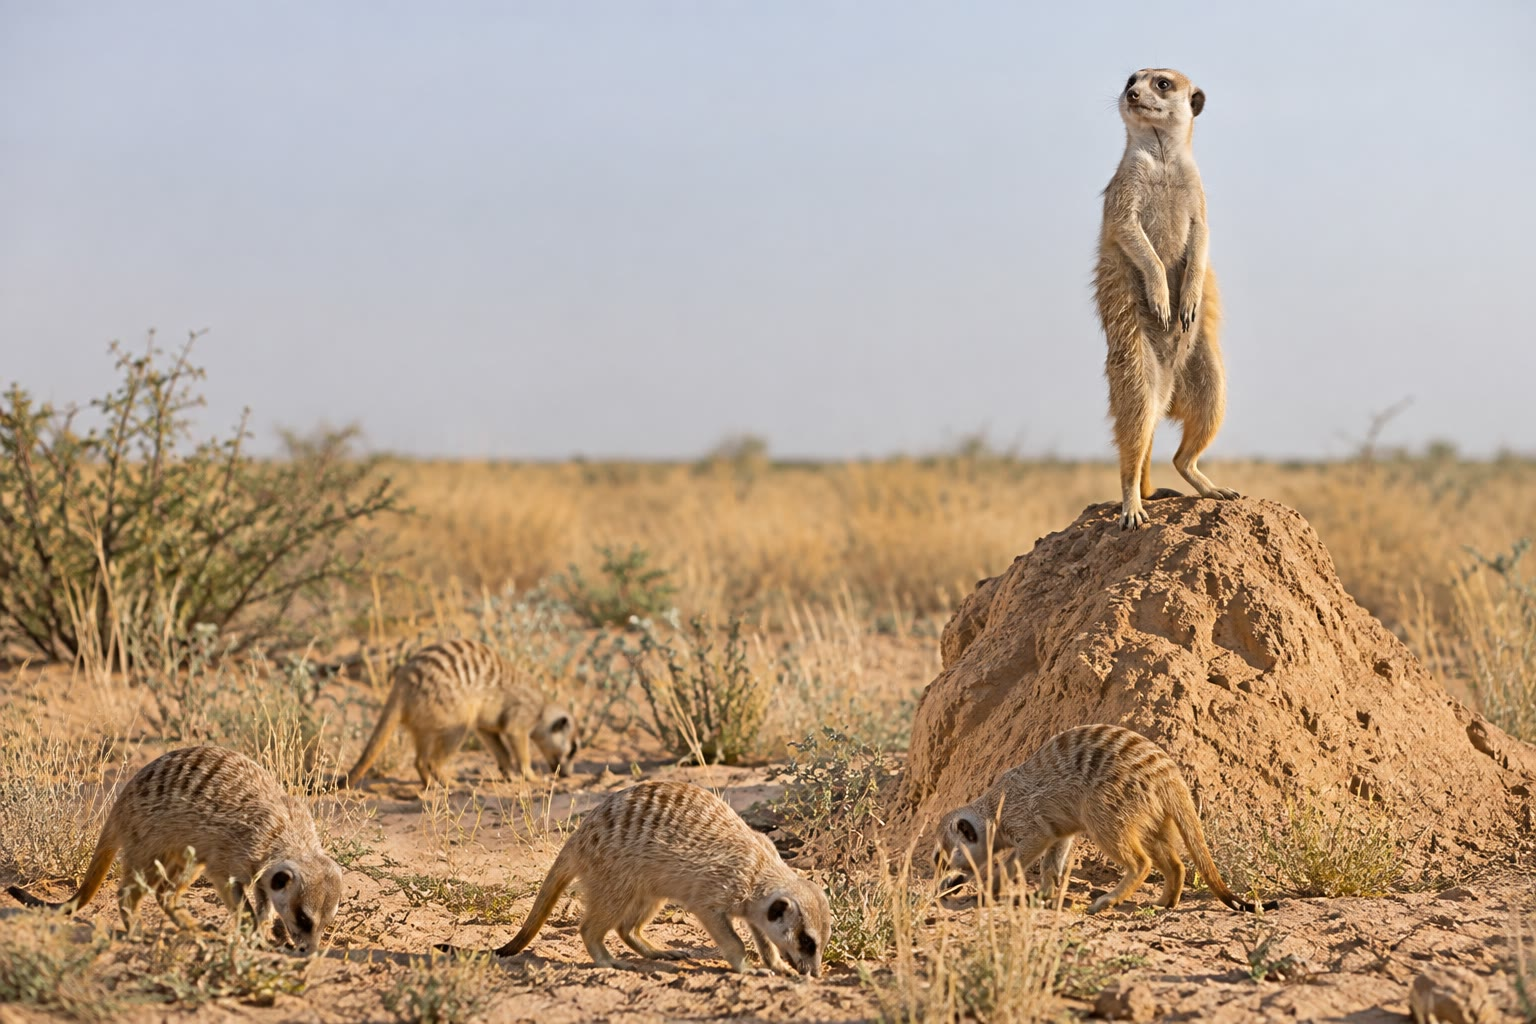
\includegraphics[width=0.46\linewidth]{images/book5/ai/b5-26-meerkat-sentinel.jpg}\hspace{0.04\linewidth}
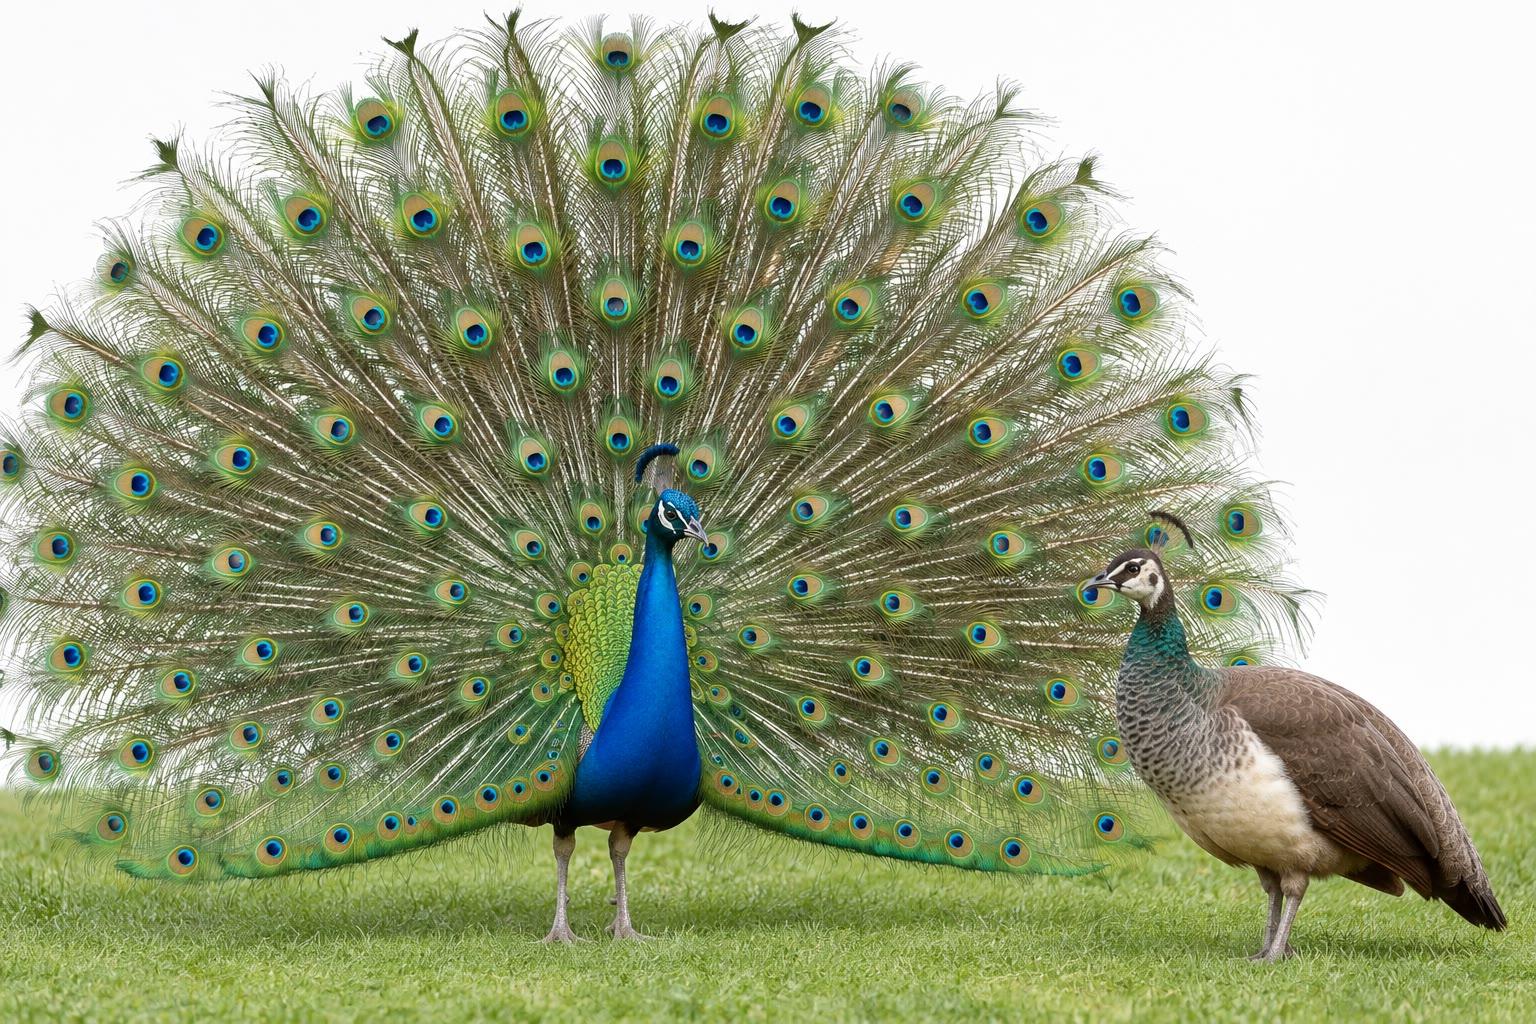
\includegraphics[width=0.46\linewidth]{images/book5/ai/b5-26-peacock-display.jpg}

{\small Kiri: seekor meerkat yang bertugas jaga di atas sebuah kelompok kerabatnya
yang sedang mencari makan. Kanan: seekor merak jantan yang memamerkan diri kepada seekor merak betina --- yakni sebuah struktur yang
berongkos makanan dan kecepatan bagi pengusungnya lalu membelikannya tiada lain selain
perhatian betinanya.}
\end{omfigure}

\section{Pasangan dan pesan}

\begin{definition}[Seleksi seksual]\label{def:b3:behavioural-ecology:sexual-selection}
\index{seleksi seksual}\index{landaian Bateman}\index{seleksi lari kencang}%
\index{asas rintangan}\index{gen baik}\index{pertentangan seksual}
Mekanisme kedua Darwin: yakni seleksi pada sifat yang memenangkan pasangan alih-alih
ketahanan hidup. Akarnya adalah anisogami --- perkembangbiakan seekor betina
dibatasi telur yang dapat dibuat dan dibekalinya, perkembangbiakan seekor jantan oleh betina
yang dapat dibuahinya --- sehingga pada kebanyakan spesies kebugaran seekor jantan naik
curam seiring cacah perkawinannya dan kebugaran seekor betina nyaris tidak (yakni
\emph{landaian Bateman}); jantannya lalu bersaing memperebutkan betinanya dan betinanya
memilih di antara jantannya. Persaingannya memberi tanduk, ranggah, gading, ukuran
besar, serta perlawanan bagian sebelumnya. Pilihannya memberi hiasan,
dan tiga keterangan mengapa betinanya lebih menyukainya. \emph{Lari kencang} milik Fisher:
sebuah kesukaan pada sebuah ekor yang sedikit lebih panjang dan ekor yang lebih panjang itu menyebar
bersama-sama, dengan masing-masing menjadikan yang lain menguntungkan, sampai ongkos ekornya pada
ketahanan hidupnya mengimbangi perolehannya pada perkawinannya. \emph{Rintangan} milik Zahavi: sebuah
hiasan yang hanya dapat ditumbuhkan seekor jantan yang sehat adalah sebuah \omterm{prop:b3:behavioural-ecology:signals}{isyarat
jujur} tentang keadaannya, justru karena ia mahal --- seekor merak
dengan sebuah kereta penuh, terbukti, punya lebih sedikit parasit. \emph{Gen baik}
dan \emph{manfaat langsung}: betinanya beroleh untung, lewat pewarisan keturunannya
atau lewat wilayah dan makanan yang disediakan jantannya.
Kepentingan kedua jenis kelaminnya berbeda, dan \emph{pertentangan seksual} --- tentang
kekerapan perkawinannya, tentang siapa yang merawat anaknya, tentang nasib sperma
pasangan sebelumnya --- adalah sebuah perlombaan senjata yang dijalankan di dalam sebuah spesies:
cairan mani lalat buah jantan memendekkan hidup betinanya lalu
menaikkan peneluran betinanya, dan betinanya mengevolusikan kekebalannya.
\end{definition}

\begin{proof}[Bukti eksperimental]
Andersson (1982) memotong lalu merekatkan bulu ekor burung janda
berekor panjang jantan di Kenya: jantan yang ekornya dipanjangkan sampai dua kali panjang
alaminya menarik empat kali lebih banyak sarang baru ke wilayahnya daripada
jantan yang ekornya dipendekkan, sementara kendali yang ekornya dipotong lalu
direkatkan kembali tanpa perubahan tidak terpengaruh --- yakni kesukaan betina pada sebuah ekor yang
lebih panjang daripada yang ditumbuhkan jantan mana pun, yakni tanda tangan sebuah kesukaan yang terpilih melampaui
sifatnya. Petrie (1994) menemukan bahwa merak betina kawin dengan jantan yang
keretanya mengusung bintik mata terbanyak, dan bahwa anak jantan itu bertahan hidup
lebih baik di hutan tempat mereka dilepaskan --- yakni sebuah manfaat \omterm{def:b3:behavioural-ecology:sexual-selection}{gen baik} yang
terukur. Bateman (1948) mencacah perkawinan dan keturunan lalat buah
yang mengusung mutasi penanda lalu menemukan landaian yang memakai namanya:
keberhasilan perkembangbiakan jantannya naik linear seiring perkawinannya, dan
keberhasilan betinanya mendatar sesudah satu.
\end{proof}

\begin{proposition}[Isyarat jujur]\label{prop:b3:behavioural-ecology:signals}
\index{komunikasi}\index{isyarat jujur}\index{tarian goyang}\index{isyarat rujukan}
Sebuah isyarat adalah sebuah tindakan yang mengubah perilaku seorang penerima dan berevolusi untuk
melakukannya; ia mantap hanya bila berbalas bagi kedua pihaknya, secara rata-rata, untuk mengirim
dan untuk menanggapi. Tempat keduanya punya kepentingan bersama, isyaratnya dapat
murah dan cermat: \emph{\omterm{prop:b3:behavioural-ecology:signals}{tarian goyang}} seekor lebah madu pencari makan (von
Frisch, dasawarsa 1940-an) menyandi arah sebuah sumber makanan sebagai sudut
lari goyangnya terhadap tegaknya --- yakni sudut sumbernya terhadap mataharinya
--- dan jaraknya sebagai lama larinya, sekitar sedetik tiap
kilometer, lalu merekrut lebah yang terbang sampai dalam beberapa puluh meter dari
sasarannya; monyet vervet memberi seruan bahaya yang berbeda bagi macan tutul, elang,
dan ular, dan pendengarnya menanggapi dengan sesuai tiap seruan yang diputar
dari sebuah pengeras suara yang tersembunyi --- yakni isyarat \emph{rujukan}. Tempat kepentingannya
bertentangan, sebuah isyarat harus mahal atau tak terpalsukan agar tetap jujur ---
raungan seekor rusa merah jantan, yang lajunya hanya dapat ditahan seekor jantan yang bugar;
besar kuakan seekor kodok, yang ditetapkan tubuhnya; hiasan paragraf
sebelumnya --- atau ia dimanfaatkan: kunang-kunang sebuah marga meniru
kilatan betina marga lain untuk memakan jantan yang datang, dan bayi
burung kukuk mengemis melampaui bayi inangnya sendiri. Teori pengisyaratan dengan demikian meramalkan
bentuk sebuah isyarat dari hubungan antarpihaknya: murah dan
memberi keterangan di antara kerabat dan pasangan yang kepentingannya berimpit, mahal dan
terupacarakan antarsaingan, serta sebuah perlombaan senjata antara pemangsa dan mangsanya.
\end{proposition}
\admitted

\begin{omfigure}
\begin{tikzpicture}[every node/.style={font=\scriptsize}, >=stealth]
  % field view
  \node[above] at (0,3.2) {di lapangan};
  \draw[->, thick, gray] (0,0) -- (0,2.6) node[above, font=\tiny] {ke arah mataharinya};
  \fill[omDef!60] (0,0) circle (0.12); \node[below, font=\tiny] at (0,-0.2) {sarang};
  \draw[->, very thick, omThm] (0,0) -- ({2.4*sin(40)},{2.4*cos(40)}); \node[right, font=\tiny, omThm] at ({2.4*sin(40)},{2.4*cos(40)}) {makanan, \qty{1}{km}};
  \draw[omThm] (0,1.0) arc[start angle=90, end angle=50, radius=1.0]; \node[font=\tiny, omThm] at (0.55,1.25) {$40^{\circ}$};
  % comb view
  \begin{scope}[shift={(6.2,0)}]
    \node[above] at (0,3.2) {pada sisir yang tegak};
    \draw[very thick, gray!60] (-1.8,-0.4) rectangle (1.8,3.0);
    \draw[->, thick, gray] (0,0) -- (0,2.6) node[above, font=\tiny] {atas (= matahari)};
    \draw[->, very thick, omThm] (0,0) -- ({1.6*sin(40)},{1.6*cos(40)}); \node[below, align=center, font=\tiny, omThm] at (0,-0.5) {lari goyang: $40^{\circ}$ dari tegaknya;\\lamanya $\approx \qty{1}{s}$ tiap km};
    \draw[omThm, dashed] ({1.6*sin(40)},{1.6*cos(40)}) .. controls (1.3,0.4) and (0.5,-0.3) .. (0,0);
    \draw[omThm, dashed] ({1.6*sin(40)},{1.6*cos(40)}) .. controls (-0.2,1.2) and (-0.6,0.3) .. (0,0);
    \draw[omThm] (0,0.8) arc[start angle=90, end angle=50, radius=0.8]; \node[font=\tiny, omThm] at (0.45,1.0) {$40^{\circ}$};
  \end{scope}
  \node[right, align=left] at (9.2,1.3) {sebuah sandi lambang: gravitasinya\\mewakili mataharinya, waktunya\\mewakili jaraknya; lebah rekrutannya tiba\\dalam puluhan meter};
\end{tikzpicture}

{\small \omterm{prop:b3:behavioural-ecology:signals}{Tarian goyang}. Sudut larinya terhadap tegaknya adalah
sudut makanannya terhadap mataharinya; panjang larinya adalah jaraknya. Sebuah isyarat
yang semurah dan secermat ini mungkin karena sang penari dan
penontonnya adalah saudari yang berkepentingan sama.}
\end{omfigure}

\begin{omfigure}
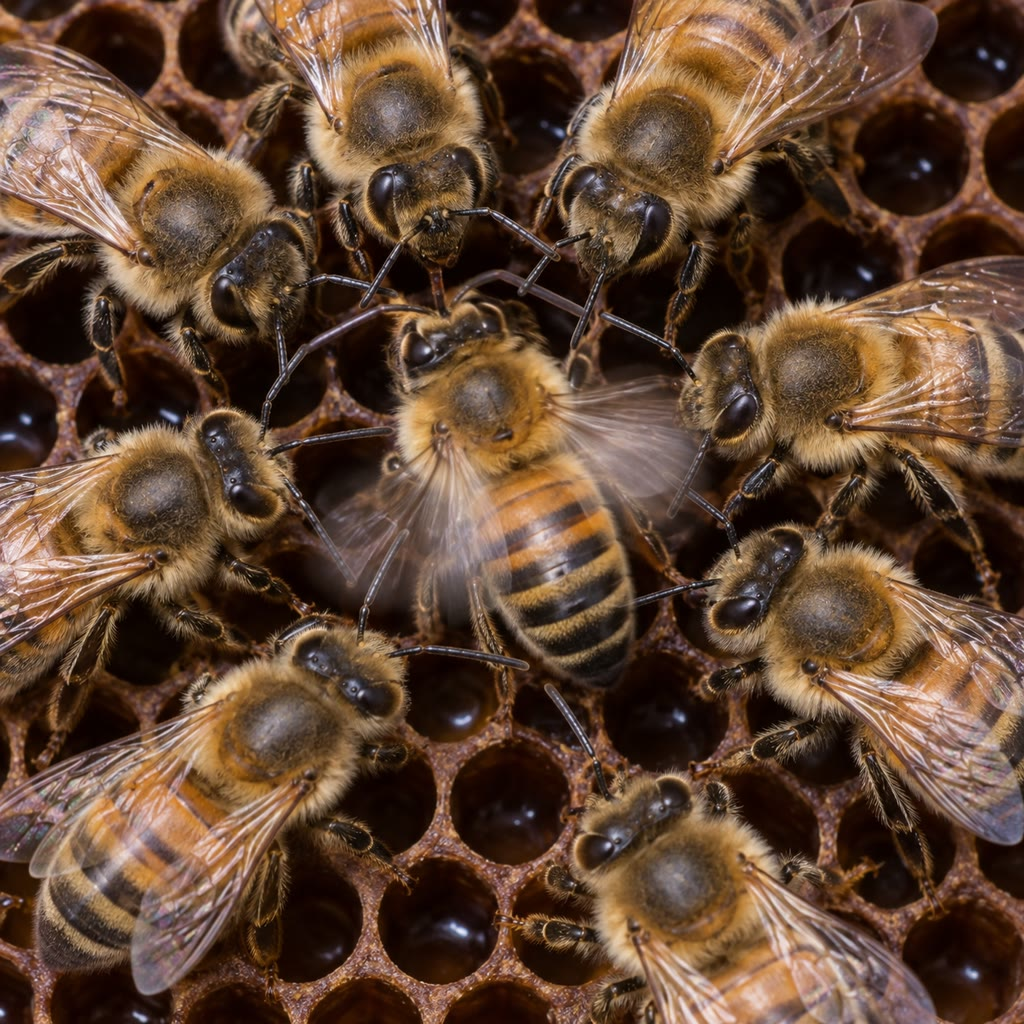
\includegraphics[width=0.4\linewidth]{images/book5/ai/b5-26-bee-dance.jpg}

{\small Seekor pencari makan yang menari di atas sisirnya, dikelilingi pekerja yang membaca
sudut dan tempo larinya.}
\end{omfigure}

\begin{remark}[Mengapa hewan tampak menghitung]\label{rem:b3:behavioural-ecology:remark}
Gelatik besarnya tidak menurunkan $g(t)/(\tau + t)$, meerkatnya tidak
menghitung $r$, dan merak betinanya tidak pernah mendengar tentang sebuah rintangan. Masing-masing
mengusung kaidah --- tinggalkanlah ketika tangkapannya melambat, serulah ketika kelompoknya
keluarga, pilihlah yang paling cemerlang --- yang telah dibentuk seleksi sebab
hewan yang mengikutinya meninggalkan lebih banyak keturunan; matematikanya milik kita,
yakni sebuah cara menanyakan apa yang harus dicapai kaidahnya agar demikian, dan
meramalkan perilakunya pada keadaan yang tidak pernah dijumpai hewannya. Ketika
ramalannya gagal --- gelatiknya tinggal terlalu lama, atau ongkos penjaganya
lebih kecil daripada yang diduga --- kegagalannya memberi keterangan: sebuah \omterm{thm:b3:behavioural-ecology:mvt}{mata uangnya}
salah, sebuah kekangannya terlewat, seorang kerabatnya salah dicacah. Pokoknya
adalah sebuah percakapan dasawarsa demi dasawarsa antara sebuah buku catatan lapangan dan
sebaris aljabar, dan keempat pertanyaan yang diajukan Tinbergen tetap menjadi
kerangka bagi keduanya.
\end{remark}

\section{Latihan}

\begin{exercise}[$\star$]\label{exo:b3:behavioural-ecology:1}
Nyatakanlah keempat pertanyaan Tinbergen lalu jawablah masing-masing, dalam sebuah kalimat, bagi
\omterm{prop:b3:behavioural-ecology:signals}{tarian goyangnya}.
\end{exercise}

\begin{exercise}[$\star$]\label{exo:b3:behavioural-ecology:2}
Apa itu sebuah \omterm{def:b3:behavioural-ecology:tinbergen}{pola tindakan tetap} dan sebuah \omterm{def:b3:behavioural-ecology:tinbergen}{rangsang tanda}? Berilah dua contoh
lalu jelaskanlah apa yang ditunjukkan tongkat ``supernormal'' bergaris merah tiga itu.
\end{exercise}

\begin{exercise}[$\star$]\label{exo:b3:behavioural-ecology:3}
Dengan kata-kata, apa yang dikatakan \omterm{thm:b3:behavioural-ecology:mvt}{teorema nilai marginal}, dan apa yang
diramalkannya tentang pemakaian petaknya ketika waktu perjalanannya berlipat dua?
\end{exercise}

\begin{exercise}[$\star$]\label{exo:b3:behavioural-ecology:4}
Definisikanlah sebuah SME. Mengapa sebuah populasi Merpati murni bukanlah SME, dan mengapa
campuran Elang--Merpatinya merugikan semua orang?
\end{exercise}

\begin{exercise}[$\star\star$]\label{exo:b3:behavioural-ecology:5}
Elang--Merpati dengan $V = 6$, $C = 10$: hitunglah $p^{*}$, hasil tiap
siasatnya pada SME-nya, dan hasil yang akan dipunyai sebuah populasi Merpati
seluruhnya. Ulangilah bagi $V = 12$, $C = 10$.
\end{exercise}

\begin{exercise}[$\star\star$]\label{exo:b3:behavioural-ecology:6}
Sebuah fungsi perolehan $g(t) = A(1 - \mathrm{e}^{-t/T_{0}})$ dengan $T_{0} =
\qty{2}{min}$. Temukanlah $t^{*}$ bagi $\tau = 2$ dan $\tau = 8$ menit (pakailah
nilai babnya), pecahan tiap petaknya yang dimakan, dan
laju jangka panjangnya $R$ sebagai sebuah pecahan $A$ tiap menit.
\end{exercise}

\begin{exercise}[$\star\star$]\label{exo:b3:behavioural-ecology:7}
Hitunglah $r$ antara: saudara tiri; kakek dan cucu; sepupu
pertama; seekor pekerja haplodiploid dan saudara jantannya; seekor ratu haplodiploid
dan anak jantannya. Jelaskanlah kedua yang terakhir.
\end{exercise}

\begin{exercise}[$\star\star$]\label{exo:b3:behavioural-ecology:8}
Sebuah seruan bahaya berongkos peluang mati \qty{2}{\%} bagi penyerunya lalu menyelamatkan
tiap dari $n$ kerabat di dekatnya dari sebuah peluang \qty{1}{\%}. Bagi $n$ yang mana
\omterm{thm:b3:behavioural-ecology:hamilton}{kaidah Hamilton} memihak seruannya bila kerabatnya adalah saudara kandung penuh?
Kemenakan? Yang tak berkerabat?
\end{exercise}

\begin{exercise}[$\star\star$]\label{exo:b3:behavioural-ecology:9}
Ekor seekor burung janda \qty{50}{cm}; bila dipanjangkan sampai \qty{75}{cm} ia
menarik dua kali sarangnya, bila dipendekkan sampai \qty{25}{cm} separuhnya. Bila ketahanan hidupnya
turun \qty{20}{\%} tiap \qty{25}{cm} yang ditambahkan, ekor yang mana yang memaksimumkan
hasil kali perkawinan dan ketahanan hidupnya, dan mengapa ekor alaminya mungkin
lebih pendek daripada itu?
\end{exercise}

\begin{exercise}[$\star\star\star$]\label{exo:b3:behavioural-ecology:10}
Tambahkanlah sebuah siasat ketiga, Pembalas, yang memamerkan diri seperti seekor Merpati tetapi
melawan bila diserang. Tulislah hasilnya terhadap Elang, Merpati, dan
dirinya sendiri (terhadap Elang ia bertarung: $(V - C)/2$; terhadap Merpati dan
Pembalas ia berbagi: $V/2$). Tunjukkanlah bahwa sebuah populasi Pembalas
tidak dapat diserbu Elang ketika $V < C$, lalu bahaslah apakah Merpati dapat
hanyut masuk.
\end{exercise}

\begin{exercise}[$\star\star\star$]\label{exo:b3:behavioural-ecology:11}
Pada sebuah perang menguras, tiap pelawannya bertahan selama sebuah waktu yang ditarik dari
sebuah sebaran; SME-nya eksponensial dengan rata-rata $V/$(ongkos tiap satuan
waktu). Jelaskanlah mengapa sebuah waktu ketahanan yang tetap tidak dapat menjadi sebuah SME, dan mengapa
sebuah sebaran eksponensial membuat harapan ketahanan lanjutan seorang
lawan yang masih memamerkan diri tak bergantung pada berapa lama ia telah
memamerkan diri.
\end{exercise}

\begin{exercise}[$\star\star\star$]\label{exo:b3:behavioural-ecology:12}
Hujah Hamilton bagi haplodiploidi meramalkan pekerjanya mestinya lebih suka
membesarkan saudari ($r = 3/4$) daripada saudara jantan ($r = 1/4$), sedangkan ratunya
menilai anak jantan dan anak perempuannya sama. Ramalkanlah nisbah kelamin
reproduktif yang mestinya dihasilkan sebuah koloni bila pekerjanya mengendalikannya, dan bila
ratunya; katakanlah apa yang ditemukan Trivers dan Hare, dan apa yang dilakukan seekor ratu yang
kawin dengan beberapa jantan terhadap hujahnya.
\end{exercise}

\section{Soal: Aritmetika Sang Penjaga}

\begin{problem}[{Soal akhir pekan --- sehari pada sebuah kelompok meerkat yang dikerjakan sebagai
ekologi perilaku: waktu petak teorema nilai marginalnya,
perlawanan permainan Elang--Merpati dan SME-nya, penghitungan kerabat
tugas penjagaan dan sebuah sarang haplodiploid, serta ongkos sebuah hiasan,
berakhir pada waktu tinggal di petaknya, kekerapan Elangnya, dan
ambang Hamilton sang penjaganya}]
\label{pb:b3:behavioural-ecology:1}
Data: petak pencarian makan dengan $g(t) = A(1 - \mathrm{e}^{-t/T_{0}})$, $T_{0}
= \qty{3}{min}$, $A = \qty{60}{kJ}$; perjalanan antarpetaknya $\tau =
\qty{3}{min}$ (habitat rapat) atau \qty{12}{min} (jarang). Perlawanan memperebutkan
sebuah liang: $V = 10$, $C = 30$ (satuan kebugaran). Penjaga: sejam bertugas
berongkos $c = 0.03$ setara keturunan bagi penjaganya (makan yang hilang,
pemaparan); ia menurunkan risiko pemangsaan tiap anggota kelompoknya, senilai $b = 0.01$
setara keturunan masing-masing; kelompoknya punya $n$ anggota berkekerabatan rata-rata $\bar r$. Sarang: seekor
pekerja dapat membesarkan entah $k$ saudari atau $k$
anak perempuannya sendiri dengan upaya yang sama. Hiasan: panjang ekor $L$ memberi
perkawinan $m(L) = L/20$ dan ketahanan hidup $s(L) = 1 - (L/100)^{2}$, dengan $L$ dalam cm.

\medskip
\noindent\textbf{Bagian I --- Petaknya.}
\begin{enumerate}
  \item Tulislah laju jangka panjangnya $R(t)$ dan syarat nilai marginalnya
        bagi $g$ ini.
  \item Tunjukkanlah bahwa syaratnya menyusut menjadi $(\tau + t)/T_{0} = \mathrm{e}^{t/T_{0}}
        - 1$, lalu selesaikanlah bagi $\tau = T_{0}$ (cobalah $t = 1.15\,T_{0}$).
  \item Selesaikanlah bagi $\tau = 4T_{0}$ (cobalah $t = 2.0\,T_{0}$).
  \item Bagi tiap halnya: berapa waktu tinggalnya dalam menit, berapa tenaga tiap petaknya,
        berapa pecahan petaknya yang dimakan, dan berapa lajunya $R$ dalam kJ/min?
  \item Sebuah kaidah praktis: ``tinggalkanlah sesudah \qty{5}{min} yang tetap.'' Hitunglah
        $R$ bagi kedua habitatnya lalu bandingkanlah dengan optimumnya. Cukup baikkah
        kaidahnya?
  \item Kaidah lain: ``tinggalkanlah ketika \qty{20}{s} berlalu tanpa sebuah
        tangkapan.'' Jelaskanlah mengapa kaidah waktu-menyerah ini menghampiri
        teoremanya, dan pada arah mana ia gagal ketika petaknya berbeda
        kekayaannya.
\end{enumerate}

\medskip
\noindent\textbf{Bagian II --- Perlawanannya.}
\begin{enumerate}[resume]
  \item Tulislah matriks hasilnya lalu hitunglah $p^{*}$.
  \item Berapa hasil bagi Elang dan bagi Merpati ketika $p = 0.1$, $p = p^{*}$, dan $p =
        0.6$; siasat mana yang menyebar pada tiap halnya?
  \item Berapa hasilnya pada SME-nya; bandingkanlah dengan hasil Merpati seluruhnya. Berapa banyak
        yang hilang dari populasinya tiap perlawanan karena kemungkinan
        bertarungnya?
  \item Sebuah kemarau menaikkan $V$ menjadi $40$ (liangnya langka). Berapa SME barunya? Apa
        yang diramalkannya tentang perkelahian pada tahun yang sukar?
  \item Borjuis: ``Elang bila penghuni, Merpati bila penyusup,'' dengan tiap perannya
        separuh waktunya. Hasilnya terhadap dirinya sendiri adalah $V/2$ tanpa
        perkelahian. Tunjukkanlah Elang tidak dapat menyerbu sebuah populasi Borjuis ketika $V
        < C$, lalu jelaskanlah kupu-kupu kayu berbintiknya.
  \item Jelaskanlah dalam sebuah kalimat mengapa kebergantungan kekerapannya, dan bukan sebuah
        optimum, yang mengatur perilaku ini.
\end{enumerate}

\medskip
\noindent\textbf{Bagian III --- Kerabat.}
\begin{enumerate}[resume]
  \item \omterm{thm:b3:behavioural-ecology:hamilton}{Kaidah Hamilton} bagi penjaganya: berapa syaratnya pada $n\bar r$? Bagi
        $n\bar r$ yang mana tugasnya berbalas?
  \item Sebuah kelompok beranggota $n = 8$ saudara kandung penuh ($\bar r = 1/2$): berbalaskah ia?
        Sebuah kelompok beranggota 8 hewan tak berkerabat? Sebuah kelompok beranggota 8 saudara tiri?
  \item Penjaganya bergizi baik, sehingga $c$-nya turun menjadi $0.01$. Berapa ambangnya
        sekarang? Mengapa hal ini meramalkan bahwa penjaganya adalah individu
        yang bergizi baik?
  \item Sarangnya: berapa nilai \omterm{thm:b3:behavioural-ecology:hamilton}{kebugaran inklusif} $k$ saudari terhadap $k$
        anak perempuan? Mana yang mestinya lebih disukai seekor pekerja, dengan nisbah berapa?
  \item Ratunya telah kawin dengan tiga jantan secara sama: berapa kekerabatan rata-rata
        pekerjanya dengan saudarinya? Bertahankah kesukaannya?
  \item Jelaskanlah mengapa \omterm{thm:b3:behavioural-ecology:hamilton}{kaidah Hamilton} tidak menuntut pelakunya
        mengenali kerabatnya, dan kaidah praktis apa yang mungkin sebenarnya dipakai seekor tupai tanah.
\end{enumerate}

\medskip
\noindent\textbf{Bagian IV --- Hiasan.}
\begin{enumerate}[resume]
  \item Kebugarannya $W(L) = m(L)\,s(L)$. Hitunglah $W$ bagi $L = 20$, $40$, $60$,
        $80$.
  \item Temukanlah $L$ yang memaksimumkan $W$ secara analitis, dan $W$ di sana.
  \item Ongkos ketahanan hidupnya mencuram menjadi $s = 1 - (L/70)^{2}$ (seekor pemangsa
        tiba). Berapa optimum barunya? Ke arah mana, dan mengapa hal ini
        meramalkan evolusi ekornya menjejaki pemangsaannya?
  \item Percobaan Andersson melipatduakan ekornya menjadi \qty{75}{cm} lalu melipatduakan
        sarangnya. Apakah kesukaan betinanya pada ekor yang lebih panjang ``melampaui
        optimumnya'' sesuai dengan keterangan lari kencangnya, keterangan rintangannya,
        atau keduanya?
  \item Mengapa sebuah hiasan yang murah bukanlah sebuah \omterm{prop:b3:behavioural-ecology:signals}{isyarat jujur}, dan bagaimana
        ongkos pada pertanyaan~21 menjadikannya \omterm{prop:b3:behavioural-ecology:signals}{isyarat jujur}?
  \item \omterm{def:b3:behavioural-ecology:sexual-selection}{Landaian Bateman}: jantannya beroleh $0.8$ keturunan tiap perkawinan tambahan,
        betinanya $0.1$. Jelaskanlah dalam sebuah paragraf bagaimana ketaksetangkupan ini
        menghasilkan baik perlawanan Bagian~II maupun hiasan
        Bagian~IV.
  \item Ringkaslah: $t^{*}$ pada habitat yang rapat (pertanyaan~4), $p^{*}$
        (pertanyaan~7), dan ambang $n\bar r$ sang penjaganya
        (pertanyaan~13).
\end{enumerate}
\end{problem}
